\chapter{Feature Evaluation}
\label{chap:evaluation}

Having established the existing feature extraction techniques as well as the new technique proposed by this study, we now look at a method of evaluating these newly extracted features against the existing features proposed by Carlin et al. \cite{DBLP:conf/interspeech/CarlinTJH11}.

The technique consists of using DTW within the same-different speech task for every extracted feature set, then calculating an AP score per feature set using the same-different results.
This process is described fully in the following sections.

\section{Dynamic Time Warping}

Dynamic Time Warping was originally used to normalise for temporal variations between an observed vector time series and a stored template.
It has since been adapted to discover repeated segments in spoken words \cite{DBLP:conf/interspeech/CarlinTJH11}. Given two vectors $\underline{a}$ and $\underline{b}$, we calculate the cosine distance between the vectors as follows:

\begin{equation}
    \mathtt{d}(\underline{a}, \underline{b}) = 1 - \displaystyle\frac{\underline{a} \cdot \underline{b}}{{||\underline{a}||}_2 {||\underline{b}||}_2}
\end{equation}
where ${||\underline{x}||}_2$ is the L2-norm of vector $\underline{x}$.

For a two-dimensional speech feature, such as spectrograms, we calculate the cosine distance for each corresponding frame vector between two words resulting in a distance matrix with structure as follows:

\begin{equation}
    {\mathrm{dist\_mat}}_{m,n} = 
 \begin{bmatrix}
  \mathtt{d}\big(\underline{a}[0], \underline{b}[0]\big) & \mathtt{d}\big(\underline{a}[0], \underline{b}[1]\big) & \cdots & \mathtt{d}\big(\underline{a}[0], \underline{b}[n-1]\big) \\
  \mathtt{d}\big(\underline{a}[1], \underline{b}[0]\big) & \mathtt{d}\big(\underline{a}[1], \underline{b}[1]\big) & \cdots & \mathtt{d}\big(\underline{a}[1], \underline{b}[n-1]\big) \\
  \vdots  & \vdots  & \ddots & \vdots  \\
  \mathtt{d}\big(\underline{a}[m-1], \underline{b}[0]\big) & \mathtt{d}\big(\underline{a}[m-1], \underline{b}[1]\big) & \cdots & \mathtt{d}\big(\underline{a}[m-1], \underline{b}[n-1]\big)
 \end{bmatrix}
\end{equation}
with $\underline{a}$ and $\underline{b}$ the two-dimensional feature vectors of the two words, first dimension the frames and second dimension the frequencies. 

Using this distance matrix, we can calculate a DTW cost matrix by essentially finding the lowest cost path through the distance matrix.
The algorithm to calculate the cost matrix is shown in Algorithm~\ref{alg:dtw}, with only the final value of the cost matrix returned.

\begin{algorithm}
    \caption{Calculating DTW cost matrix}
    \label{alg:dtw}
    \begin{algorithmic}
        \Function{DTWDistance}{$\mathtt{dist\_mat_{m,n}}$}
        \State $\mathtt{cost\_mat} = [0\cdots n, 0\cdots m]$
        \For{$i=1$ to $n+1$}
        \State $\mathtt{cost\_mat}[i, 0] = \infty$
        \EndFor
        \For{$i=1$ to $m+1$}
        \State $\mathtt{cost\_mat}[0, i] = \infty$
        \EndFor
        \For{$i=0$ to $n-1$}
        \For{$j=0$ to $m-1$}
        \State $\mathtt{penalty} = \mathtt{argmin}(\mathtt{cost\_mat}[i, j], \mathtt{cost\_mat}[i, j + 1], \mathtt{cost\_mat}[i+1, j])$
        \State $\mathtt{cost\_mat}[i+1, j+1] = \mathtt{dist\_mat}[i, j] + \mathtt{penalty}$
        \EndFor
        \EndFor
        \State Return $\mathtt{cost\_mat[n, m]}$
        \EndFunction
    \end{algorithmic}
\end{algorithm}

This algorithm is used to define a similarity metric between two spoken word features, with a lower DTW distance expected for the same spoken word, and a higher distance for different words.

It is expected that a better feature extraction technique would more definitively separate similar spoken words from different ones.

To measure the quality of a given feature set, we calculate the DTW distance between each spoken word within the feature set, separating the distances for two of the same words and two different words \cite{kamper_elsner_jansen_goldwater_2015}.

Importantly, iteratively comparing each spoken word to every other spoken word causes the algorithm to be an $O(N^2)$ process, or more precisely it will require $(\frac{N^2-N}{2})$ comparisons, where $N$ is the number of words in the feature set, which for the Buckeye data set consisting of 2\,733 spoken words, requires 3\,733\,278 comparisons per feature set.

\section{Average Precision}

Once we have obtained two lists per feature set, one with DTW distances for similar words and one for different words, we must now determine the separability of the the scores of the two lists.
A possible solution could be to calculate a reliability coefficient for the DTW distances\cite{reliability}, but previous studies have found that skewness in the distributions could lead to instability across different feature sets \cite{DBLP:conf/interspeech/CarlinTJH11}.

Instead, an AP score was calculated by following the method proposed by Carlin et al. \cite{DBLP:conf/interspeech/CarlinTJH11}. To calculate the AP score for a given feature set, we define a threshold $\tau$ for which we assume that for two spoken word vectors, $\underline{a}$ and $\underline{b}$, the two words are the same if $\mathtt{DTW}(\underline{a}, \underline{b}) \leq \tau$. 

For a given value of $\tau$ we are able to calculate two values, namely, the precision and the recall point.
Precision is defined as the percentage of same word pairs whose DTW distance falls below the threshold, and recall is defined as the percentage of different word DTW distances that fall above the threshold.
Sweeping $\tau$ from the minimum DTW distance to the maximum distance for a given feature set allows us to draw a precision-recall curve.
A precision-recall curve for a feature set where the DTW distances are perfectly separated is shown in Figure~\ref{fig:pr-curve}, as well as the spectrograms, filterbanks and MFCCs of the Buckeye data set.

\begin{figure}[h]
    \centering
    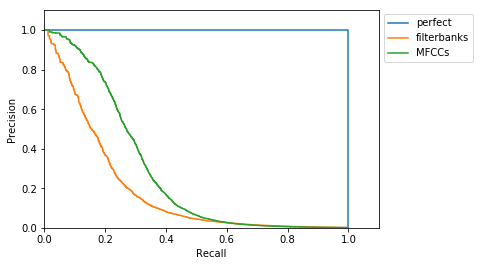
\includegraphics[width=0.8\linewidth]{content/fig/pr_curve.png}
    \caption{Precision-recall curves for a perfectly separable feature set, spectrograms, filterbanks and MFCCs for the Buckeye data set.}
    \label{fig:pr-curve}
\end{figure}

Note that for a perfect precision-recall curve, the area underneath the curve is exactly 1.
For the spectrograms, filterbanks and MFCCs, these areas are 0.02347, 0.189 and 0.2843 respectively.
The area underneath the curve thus acts as a global metric to measure the separability of a given feature set, thus implying a clear improvement in feature quality from filterbanks against spectrograms, and from MFCCs against filterbanks.
It is exactly this metric that we use as our AP score, with a score of 1 denoting a perfect feature set, and the lower the AP score, the generally more difficult it will be for a model to distinguish between words for the given feature set.

This AP score technique has been shown to correlate well with phone recognition error rates \cite{DBLP:conf/interspeech/CarlinTJH11} and has been used in several other unsupervised studies \cite{kamper_elsner_jansen_goldwater_2015}.